\documentclass[utf8]{ctexart}
\usepackage{graphicx}
\usepackage{amsmath, amssymb, amsthm}
\usepackage{geometry}
\usepackage{enumitem}
\usepackage{xcolor}
\usepackage{algorithm}
\usepackage{algpseudocode}
\usepackage{mdframed}
\usepackage{tikz}
\usetikzlibrary{graphs, positioning, arrows.meta}

\geometry{a4paper, margin=2.5cm}

% 定理环境
\newtheoremstyle{mystyle}
  {8pt}{8pt}{\kaishu}{0pt}{\bfseries}{}{1em}{}
\theoremstyle{mystyle}
\newtheorem{theorem}{定理}
\newtheorem{lemma}{引理}

% 好看的题目框
\newmdenv[
  linecolor=black!40,
  linewidth=1pt,
  backgroundcolor=gray!8,
  roundcorner=5pt,
  innertopmargin=8pt,
  innerbottommargin=8pt,
]{problembox}

\title{\textbf{离散数学2\quad 作业4}}
\date{\today}
\author{李子嘉 2024012325}
\begin{document}
\maketitle

\section*{题目1}

\begin{problembox}
请对 Warshall 算法进行适当修改，以便在计算道路矩阵后，可以查知任意两顶点间具体的路径。
\end{problembox}

\textbf{解：} Warshall 算法的核心思想是通过动态规划来更新道路矩阵。在无权图中，第k轮的$P[i][j]$表示在前k个顶点中，是否存在一条从顶点i到顶点j的路径。
从第k轮到第k+1轮，我们需要检查新加入的第$k+1$个顶点能否作为中间点连接i和j。在有权图中，对应的定义改为$P[i][j]$表示在前k个顶点中，从顶点i到顶点j的路径的最短距离。
在每一轮迭代中，我们需要改为检查新的顶点是否能减小从i到j的路径长度，即检查$P[i][k] + P[k][j] < P[i][j]$。

所以，我们只需要在每次更新时，记录是哪一个顶点k使得$P[i][j]$发生了更新，这就是目前探明的从i到j的路径上，j的前一个顶点。通过这种方式，我们可以在算法结束后，通过路径矩阵来回溯出从i到j的具体路径。
我们新定义一个矩阵$Q$，其中$Q[i][j]$表示从顶点i到顶点j的最短路径上$j$的前一个顶点。每次更新意味着通过k到j的路径更短，那么我们就把$Q[i][j]$更新为$Q[k][j]$，此时$j$的前一个顶点就是从k到j的路径上的前一个顶点。
\textbf{由于最短路径的子路径也是最短路径，我们把得到的值代入$Q[i][j]$的$j$中，就可以得到从i到j的完整路径。}
初始时，如果存在边(i, j)，则$Q[i][j] = i$，否则$Q[i][j] = -1$。我们来实现这个算法：

\begin{algorithm}[H]
\caption{改进的 Warshall 算法}
\begin{algorithmic}[1]
    \Require $P$：邻接矩阵（存储初始权重，不相连设为 $\infty$），$n$：顶点数量
    \Ensure $P$：最短路径权重矩阵，$Q$：前驱矩阵（用于回溯路径）
    
    \State \Comment{1. 初始化前驱矩阵 $Q$}
    \For{$i = 1$ to $n$}
        \For{$j = 1$ to $n$}
            \If{$i = j$ \textbf{or} $P[i][j] = \infty$}
                \State $Q[i][j] \gets -1$ \Comment{无前驱或自环}
            \Else
                \State $Q[i][j] \gets i$ \Comment{初始前驱为源点 $i$}
            \EndIf
        \EndFor
    \EndFor

    \State \Comment{2. 动态规划核心：三重循环}
    \For{$k = 1$ to $n$}
        \For{$i = 1$ to $n$}
            \For{$j = 1$ to $n$}
                \If{$P[i][k] + P[k][j] < P[i][j]$}
                    \State $P[i][j] \gets P[i][k] + P[k][j]$
                    \State $Q[i][j] \gets Q[k][j]$ \Comment{关键：继承从 $k$ 到 $j$ 的前驱节点}
                \EndIf
            \EndFor
        \EndFor
    \EndFor

    \Function{GetPath}{$i, j$} \Comment{路径回溯函数}
        \If{$Q[i][j] = -1$}
            \State \Return $[]$ \Comment{不可达}
        \EndIf
        \State $\textit{path} \gets [j]$
        \While{$j \neq i$}
            \State $j \gets Q[i][j]$ \Comment{向源点方向回溯}
            \State $\textit{path}.\text{prepend}(j)$
        \EndWhile
        \State \Return $\textit{path}$
    \EndFunction
\end{algorithmic}
\end{algorithm}

\newpage

\section*{题目2}

\begin{problembox}
分别使用 DFS 和 BFS 算法，从$v_1$开始遍历图2.41。使用 BFS 算法时写出每个集合$A_i$，使用DFS算法时写出顶点的访问顺序。
\end{problembox}

\subsection*{图2.41(a)}

\begin{center}
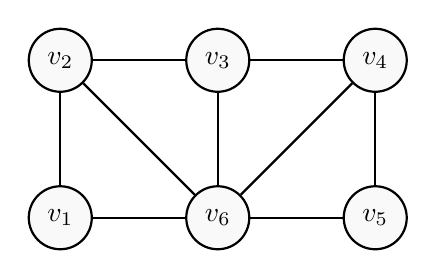
\begin{tikzpicture}[node distance={22mm}, main/.style = {draw, circle, thick, fill=gray!5, minimum size=0.8cm}] 
    % 坐标定义
    \node[main] (v1) at (0,0) {$v_1$}; 
    \node[main] (v2) at (0,2) {$v_2$}; 
    \node[main] (v6) at (2,0) {$v_6$}; 
    \node[main] (v3) at (2,2) {$v_3$}; 
    \node[main] (v5) at (4,0) {$v_5$}; 
    \node[main] (v4) at (4,2) {$v_4$}; 

    % 边定义
    \draw[thick] (v1) -- (v2);
    \draw[thick] (v1) -- (v6);
    \draw[thick] (v2) -- (v3);
    \draw[thick] (v2) -- (v6); 
    \draw[thick] (v3) -- (v6);
    \draw[thick] (v3) -- (v4);
    \draw[thick] (v6) -- (v4); 
    \draw[thick] (v6) -- (v5);
    \draw[thick] (v4) -- (v5);
\end{tikzpicture}
\end{center}

\subsubsection*{广度优先搜索}
假设邻接点按索引升序访问。使用队列 $Q$ 记录遍历状态：

\begin{table}[H]
\centering
\begin{tabular}{|c|c|l|l|}
\hline
\textbf{步骤} & \textbf{出队节点} & \textbf{当前队列状态 (Front $\to$ Rear)} & \textbf{访问序列} \\ \hline
1 & - & $[v_1]$ & $v_1$ \\ \hline
2 & $v_1$ & $[v_2, v_6]$ & $v_1, v_2, v_6$ \\ \hline
3 & $v_2$ & $[v_6, v_3]$ & $v_1, v_2, v_6, v_3$ \\ \hline
4 & $v_6$ & $[v_3, v_4, v_5]$ & $v_1, v_2, v_6, v_3, v_4, v_5$ \\ \hline
5 & $v_3$ & $[v_4, v_5]$ & $v_1, v_2, v_6, v_3, v_4, v_5$ \\ \hline
6 & $v_4$ & $[v_5]$ & $v_1, v_2, v_6, v_3, v_4, v_5$ \\ \hline
7 & $v_5$ & $[]$ & $v_1, v_2, v_6, v_3, v_4, v_5$ \\ \hline
\end{tabular}
\end{table}

\textbf{BFS 最终序列：} $v_1, v_2, v_6, v_3, v_4, v_5$
\subsubsection*{深度优先搜索}
同样遵循邻接点索引升序访问原则：

\begin{itemize}
    \item 从 $v_1$ 出发，访问其最小邻居 $v_2$。
    \item 从 $v_2$ 出发，访问其最小未访问邻居 $v_3$（注意 $v_6 > v_3$）。
    \item 从 $v_3$ 出发，访问其最小未访问邻居 $v_4$（此时 $v_6$ 仍未被访问）。
    \item 从 $v_4$ 出发，访问其最小未访问邻居 $v_5$。
    \item 从 $v_5$ 出发，访问其唯一未访问邻居 $v_6$。
    \item 此时所有顶点均已访问，算法回溯并结束。
\end{itemize}

\textbf{DFS 最终序列：} $v_1, v_2, v_3, v_4, v_5, v_6$
\subsection*{图2.41(b)}
\begin{center}
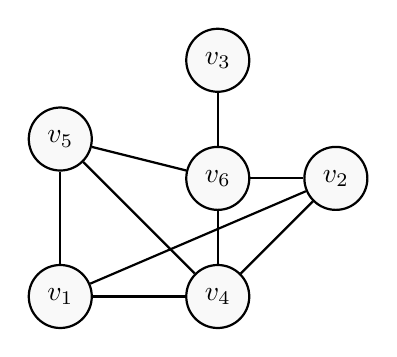
\begin{tikzpicture}[node distance={22mm}, main/.style = {draw, circle, thick, fill=gray!5, minimum size=0.8cm}] 
    % 坐标定义
    \node[main] (v1) at (0,0) {$v_1$}; 
    \node[main] (v2) at (3.5,1.5) {$v_2$}; 
    \node[main] (v6) at (2,1.5) {$v_6$}; 
    \node[main] (v3) at (2,3) {$v_3$}; 
    \node[main] (v5) at (0,2) {$v_5$}; 
    \node[main] (v4) at (2,0) {$v_4$}; 

    % 边定义
    \draw[thick] (v1) -- (v2);
    \draw[thick] (v1) -- (v4);
    \draw[thick] (v1) -- (v5);
    \draw[thick] (v2) -- (v4);
    \draw[thick] (v2) -- (v6); 
    \draw[thick] (v3) -- (v6);
    \draw[thick] (v4) -- (v5);
    \draw[thick] (v4) -- (v6);
    \draw[thick] (v5) -- (v6);
\end{tikzpicture}
\end{center}
\subsubsection*{广度优先搜索}
使用队列 $Q$ 记录状态，起始节点为 $v_1$：
\begin{table}[H]
    \centering
    \begin{tabular}{|c|c|l|l|}
        \hline\textbf{步骤} & \textbf{出队} & \textbf{队列状态 (Front $\to$ Rear)} & \textbf{访问序列} \\
        \hline1 & - & $[v_1]$ & $v_1$ \\ 
        \hline2 & $v_1$ & $[v_2, v_4, v_5]$ & $v_1, v_2, v_4, v_5$ \\ 
        \hline3 & $v_2$ & $[v_4, v_5, v_6]$ & $v_1, v_2, v_4, v_5, v_6$ \\ 
        \hline4 & $v_4$ & $[v_5, v_6]$ (邻居均已访问) & $v_1, v_2, v_4, v_5, v_6$ \\
        \hline5 & $v_5$ & $[v_6]$ (邻居均已访问) & $v_1, v_2, v_4, v_5, v_6$ \\ 
        \hline6 & $v_6$ & $[v_3]$ & $v_1, v_2, v_4, v_5, v_6, v_3$ \\ 
        \hline7 & $v_3$ & $[]$ & $v_1, v_2, v_4, v_5, v_6, v_3$ \\
        \hline
    \end{tabular}
\end{table}
\textbf{BFS 序列：} $v_1, v_2, v_4, v_5, v_6, v_3$
\subsubsection*{深度优先搜索}
\begin{enumerate}
    \item \textbf{Visit $v_1$}
    \item $\to$ \textbf{Visit $v_2$} (自 $v_1$ 的邻居 $\{v_2, v_4, v_5\}$ 中选最小)
    \item $\to$ \textbf{Visit $v_4$} (自 $v_2$ 的邻居 $\{v_4, v_6\}$ 中选最小)
    \item $\to$ \textbf{Visit $v_5$} (自 $v_4$ 的邻居 $\{v_5, v_6\}$ 中选最小)
    \item $\to$ \textbf{Visit $v_6$} (自 $v_5$ 的邻居 $\{v_6\}$ 中选最小)
    \item $\to$ \textbf{Visit $v_3$} (自 $v_6$ 的唯一未访问邻居 $\{v_3\}$)
\end{enumerate}
\textbf{DFS 序列：} $v_1, v_2, v_4, v_5, v_6, v_3$

\newpage
\section*{题目3}
\begin{problembox}
    如图2.44所示，A从顶点$v_2$出发，B从顶点$v_1$出发。要求两人遍历完所有边至少一次后到达终点$v_3$，谁更快到达谁就胜利。
    假设两人经过同一条边的时间相同，请问谁有必胜策略？
\end{problembox}
\begin{center}
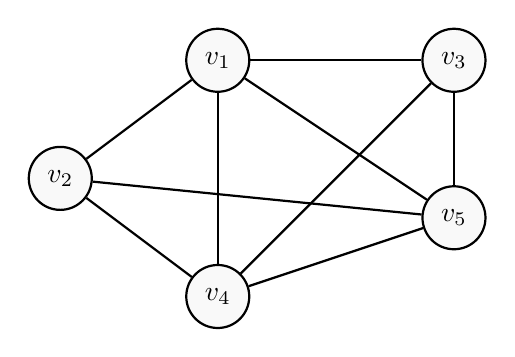
\begin{tikzpicture}[node distance={22mm}, main/.style = {draw, circle, thick, fill=gray!5, minimum size=0.8cm}] 
    % 坐标定义
    \node[main] (v1) at (0,3) {$v_1$}; 
    \node[main] (v2) at (-2,1.5) {$v_2$}; 
    \node[main] (v3) at (3,3) {$v_3$}; 
    \node[main] (v5) at (3,1) {$v_5$}; 
    \node[main] (v4) at (0,0) {$v_4$}; 

    % 边定义
    \draw[thick] (v1) -- (v2);
    \draw[thick] (v1) -- (v3);
    \draw[thick] (v1) -- (v4);
    \draw[thick] (v1) -- (v5);
    \draw[thick] (v2) -- (v4);
    \draw[thick] (v2) -- (v5); 
    \draw[thick] (v3) -- (v4);
    \draw[thick] (v3) -- (v5);
    \draw[thick] (v4) -- (v5);
\end{tikzpicture}
\end{center}
\textbf{解：} 简单观察可知，全图有2个度数为3的顶点（$v_2$ 和 $v_3$），其余顶点度数为4。由于奇数度数的顶点数量为2，因此存在欧拉道路，且必然以这两个奇数度数的顶点为起点和终点。
题目要求两人遍历完所有边至少一次后到达终点$v_3$，显然两人所花的时间可以分为两部分：第一部分是遍历所有边的时间，第二部分是从遍历完所有边的位置到达终点$v_3$的时间。

由于A的起点正好是欧拉道路的起点，所以A可以直接按照欧拉道路的顺序遍历所有边，最终停在欧拉道路的终点$v_3$，而$v_3$也是我们的目的地，所以A不需要额外的时间就可以到达终点。A的时间就是走过所有边一次的时间，是最小值。
而B的起点是偶数度数的点，从B开始必定需要重复访问某些边才能遍历完所有边，仅这部分就需要比A更多的时间。因此B不可能有必胜策略，A必胜。

A的必胜策略就是按照欧拉道路的顺序遍历所有边，我们给出一个欧拉道路的示例：$v_2 \to v_5 \to v_4 \to v_2 \to v_1 \to v_4 \to v_3 \to v_1 \to v_5 \to v_3$。

\bigskip
\section*{第4题}
\begin{problembox}
证明：若 $G=(V, E)$ 是一个二分图，即 $V(G)$ 可以划分为两个子集 $X$ 和 $Y$，使得所有的$ e=(u, v) \in E(G)$， $u$ 、 $v$都分别属于 $X$ 或 $Y$。
如果$|X|\neq|Y|$，则 $G$ 一定没有哈密顿回路。如果 $|X|-|Y|>1$，则一定没有哈密顿路径。
\end{problembox}
\textbf{解：} 我们需要一个课件里的关键引理：如果图 $G$ 有哈密顿回路，那么对于图 $G$ 任意一个子集 $S$，图 $G-S$ 的连通分量的数量不超过 $|S|$。
它的推论是：如果图 $G$ 有哈密顿路径，那么对于图 $G$ 任意一个子集 $S$，图 $G-S$ 的连通分量的数量不超过 $|S| + 1$。

对于第一问，我们假设 $G$ 有哈密顿回路，我们选择 $|X|$ 和 $|Y|$ 中较小的那个子集作为 $S$，我们不妨假设 $|X| < |Y|$，因此 $S=X$。
那么对于 $S=X$，图 $G-S$ 的连通分量的数量为 $|Y|$，而 $|Y| > |X| = |S|$，与引理矛盾，因此 $G$ 没有哈密顿回路。

对于第二问，我们假设 $G$ 有哈密顿路径，那么对于 $S=Y$，图 $G-S$ 的连通分量的数量为 $|X|$，而 $|X| > |Y| + 1 = |S| + 1$，与引理矛盾，因此 $G$ 没有哈密顿路径。
\end{document}